\section{Metrics}

\begin{frame}{Reporting Posterior Metrics}

  \begin{itemize}
    \item By the end of 1 year, we report key metrics from the final posterior distribution.
    \item 95\% Confidence Interval: The range where the product's revenue is most likely to lie.
    \item Posterior Mean: The expected revenue generated based on whole year of data.
    \item Standard Deviation: Reflects our confidence in this revenue estimate; lower Standard Deviation implies greater certainty.
  \end{itemize}
  
\end{frame}

\begin{frame}{95\% Confidence Interval}

\begin{figure}
  \centering
  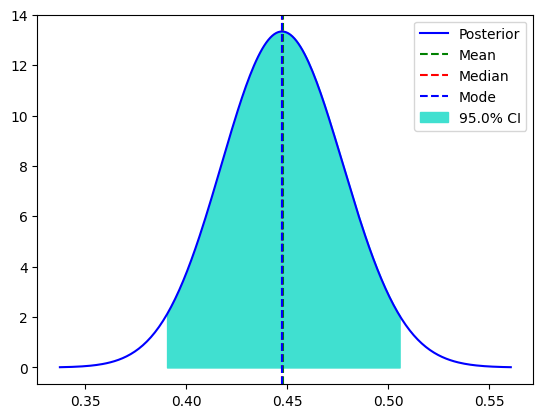
\includegraphics[width=.8\linewidth]{../Report/images/confidence-interval.png}
  \caption{95\% Confidence Interval}
\end{figure}
  
\end{frame}

\begin{frame}{Posterior Mean and Standard Deviation Analysis}

  \begin{itemize}
    \item The posterior mean over time shows how our estimate of revenue has evolved.
    \item A decreasing Standard Deviation suggests that our confidence is increasing, as we have more data to base our estimates on.
    \item These metrics help us assess how consistent the product sale has been over time.
  \end{itemize}
  
\end{frame}

\begin{frame}{Posterior Mean}
    
\begin{figure}
  \centering
  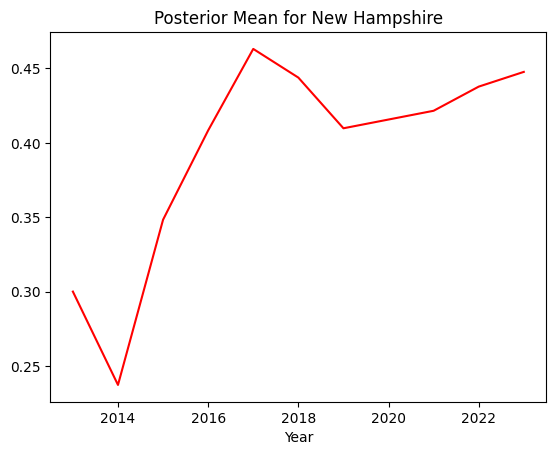
\includegraphics[width=.8\linewidth]{../Report/images/posterior-mean.png}
  \caption{Posterior Mean for each month}
\end{figure}

\end{frame}

\begin{frame}{Posterior Standard Deviation}

\begin{figure}
  \centering
  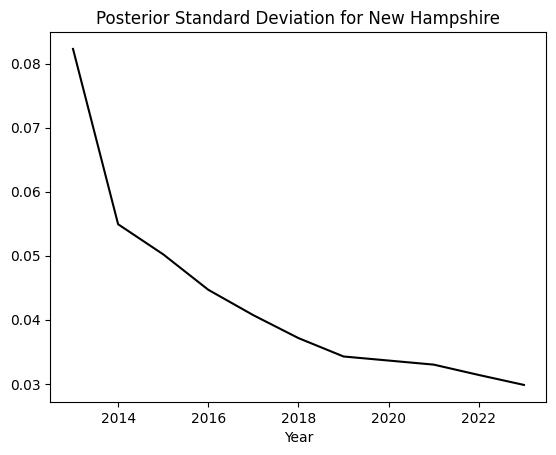
\includegraphics[width=.8\linewidth]{../Report/images/posterior-sd.png}
  \caption{Posterior Standard Deviation for each month}
\end{figure}

\end{frame}